\section{引言}

\begin{keytakeaways}
\begin{itemize}\setlength{\itemsep}{2pt}
  \item \textbf{物理图像}：Jones 多项式来自三维 Chern-Simons 型拓扑理论，Khovanov 同调来自四维拓扑理论；后者在圆上紧致化即约化为前者。因此四维的"计数椭圆方程解"应重现 Jones 多项式，而其再升一维（范畴化）应给出 Khovanov 同调。
  \item \textbf{数学工具}：N=4 超 Yang-Mills 理论中的 BPS 方程 (\ref{bpseqns})、Nahm 方程与 Nahm 极边界条件、主嵌入与正则元素、瞬子数、GNO/Langlands 对偶群。
  \item \textbf{主要结论}：配分函数由带符号地计数 BPS 方程的解给出（式~(\ref{partfn})）；当 W 取三维欧氏空间、对偶群取 SU(2) 且纽结标以二维表示时，它应成为 Jones 多项式。
  \item \textbf{方法要点}：沿 $x^1$ 方向拉伸纽结以实现三维约化，再用参数的绝热演化拼回四维图像；并借助库仑分支参数破坏规范对称性，以在低能下得到阿贝尔描述。
  \item \textbf{伏笔}：五维提升只有在 $t=\pm1$ 时才具有出人意料的四维对称性，这正是本文先取 $t=\pm1$、随后又扰动 $t$ 的原因。
\end{itemize}
\end{keytakeaways}

Jones 多项式 \cite{Jones} 是纽结的一个不变量，它与数学物理的许多方面有着多重联系，包括可积格点统计力学、二维共形场论及与之相关的辫群表示，以及三维 Chern-Simons 规范理论。Khovanov 同调 \cite{Khovanov} 是较晚近的一个四维拓扑理论；在这一理论中，纽结被看作三维空间中的一个对象，而与纽结相联系的不变量是一个（物理态的）向量空间，而不是一个数。两个理论之间的关系是：与 Khovanov 同调相联系的四维理论在圆上紧致化后，约化为给出 Jones 多项式的三维理论。

Khovanov 同调已在拓扑弦的框架内得到物理解释 \cite{GSV}，其基础是关于开弦 BPS 态的早期工作 \cite{OV}。关于更多进展的示例，见 \nocite{LMV,NV,Ma,DGR,DVV,AY,CNV,ACDKV,AgS} \cite{LMV}-\cite{AgS}。文献~\cite{fiveknots} 给出了 Khovanov 同调的另一种但密切相关的物理解释，其中可以找到关于 Jones 多项式、Khovanov 同调及其与数学物理之关系的更详细文献。

按照这一较新的提议，Jones 多项式可以通过计数四维中某些椭圆偏微分方程的解来计算，而 Khovanov 同调则可以通过计数 4+1 维中相关方程的解来构造。导出这一提议的推理依赖于四维 $\N=4$ 超 Yang-Mills 理论的电磁对偶：把一个本质上相当"量子"的描述（它与包围三维流形上的 Chern-Simons 规范理论密切相关）变换为另一个"半经典"的描述，在后一描述中，配分函数只需适当地计数某些微分方程的经典解即可算出。

与其依赖电磁对偶来预言这个或许有些神秘的结果，我们能否通过对这些方程的直接研究来理解它？这就是本文的目标。我们将对 Jones 多项式获得相当程度的理解，并为理解 Khovanov 同调打下良好的基础。

\subsection{简要回顾}\label{review}

这里所说的四维方程可以描述如下。规范群是一个紧李群\footnote{我们颠倒了 \cite{fiveknots} 中的记号：把 Chern-Simons 描述中的规范群记作 $G^\vee$，而把对偶的"磁性"描述中的规范群记作 $G$，本文关注的正是后者。}   $G$。方程中的场包括一个规范场 $A$，它是 $G$-丛 $E\to \MM$ 上的联络，其中 $\MM$ 是一个有向黎曼四维流形；还包括另一个场 $\phi$，它是取值于 $G$ 的伴随表示的一形式。这些方程最初是在与几何 Langlands 对应相关的研究中提出的 \cite{KW}，它们为
\begin{align}\label{bpseqns} (F-\phi\wedge \phi + \t \,\d_A\phi)^+&=0   \cr
                             (F-\phi\wedge\phi-\t^{-1}\d_A\phi  )^- &=0 \cr
                               \d_A\star\phi&=0,                     \end{align}
其中两形式 $b$ 的自对偶与反自对偶投影分别记作 $b^\pm$；$\d_A=\d+[A,\,\cdot\,]$ 是规范协变外微分；$F=\d A+A\wedge A$ 是 Yang-Mills 场强；$\star$ 是 Hodge 星号算子；$\t$ 是一个实参数。（实际上，$\t$ 取值于 $\mathbb{RP}^1=\mathbb{R}\cup\infty$；当 $\t\to 0$ 或 $\t\to\infty$ 时，需将第二个方程乘以 $\t$，或将第一个方程乘以 $\t^{-1}$。）为研究纽结不变量，我们取 $\MM=W\times \R_+$，其中 $W$ 是一个三维流形，$\R_+$ 是半直线 $y\geq 0$（图~\ref{knotboundary}）。
% [Tutor Note: 易错点] 自对偶/反自对偶投影的符号约定为 b^± = (b ± ⋆b)/2（以 ⋆² = +1 于两形式上的黎曼度量为前提）；若采用相反的 ± 约定，式 (\ref{bpseqns}) 中 t 与 t^{-1} 的角色会互换，核对时务必回到原文定义。另注意 t 并非普通实数参数，而是射影直线 RP¹ 上的点：t→0 与 t→∞ 处的方程须分别乘以 t 或 t^{-1} 才能取到有限的极限，直接令 t=0 会丢失一个方程。

\begin{figure}
 \begin{center}
     % >>> 原文图 1（原稿第 5 页）
  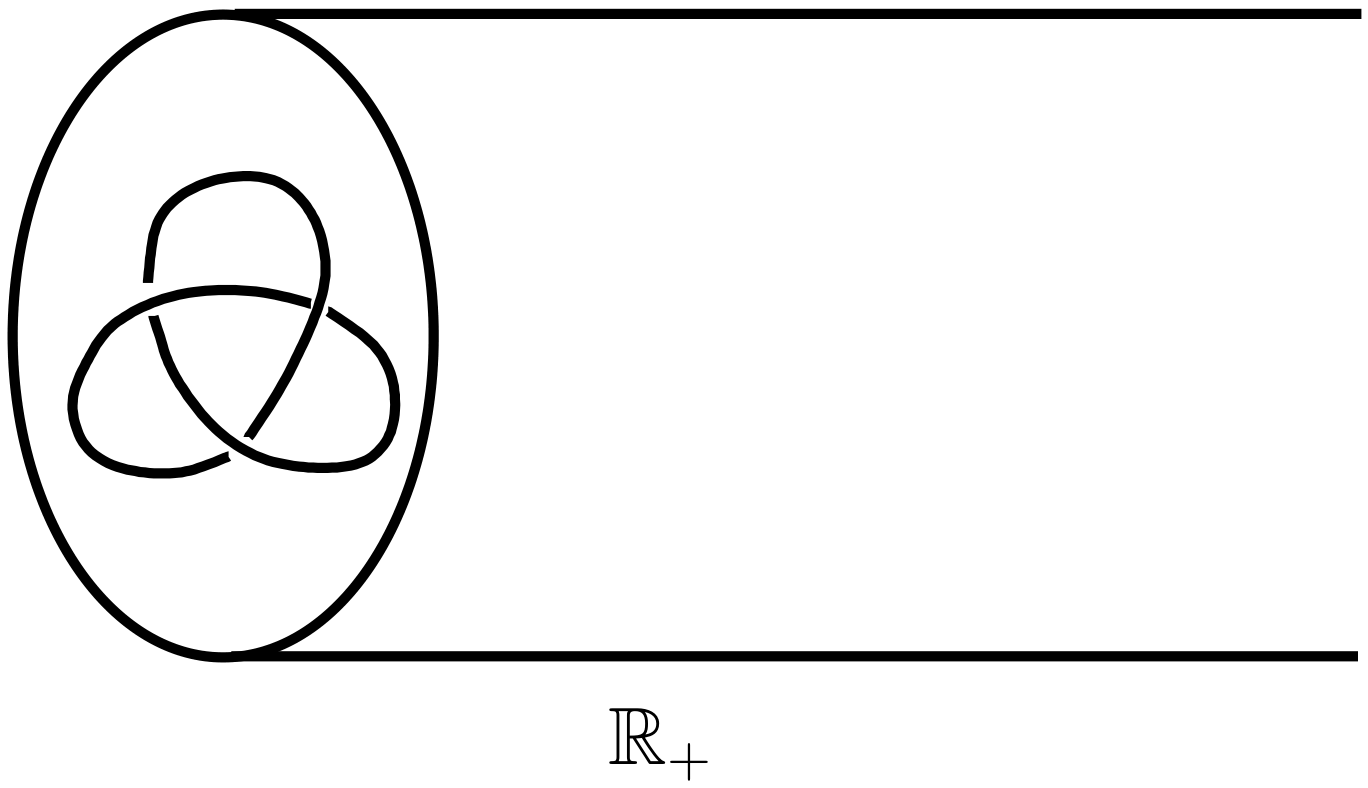
\includegraphics[width=3.5in]{figs/Fig01.png}
 \end{center}
\caption{\small  一个纽结被置于四维流形 $\MM=W\times\R_+$ 的边界上。（原稿第 5 页）}
 \label{knotboundary}
\end{figure}



$y=0$ 处的边界条件略显微妙，但在没有纽结的情形下可以很容易地描述。先假设 $\t=1$。由于边界条件是局域的，我们在描述它时不妨取 $W=\R^3$。（无论如何，这正是本文的主要例子。）考虑一个在沿 $\R^3$ 的平移下不变、且 $A$ 与 $\phi$ 垂直于边界的分量均为零的经典解。此时方程约化为关于 $\vec\phi$——即 $\phi$ 与边界相切的部分——的 Nahm 方程：
\begin{equation}\label{nahm}\frac{\d \vec\phi}{\d y}+\vec\phi\times \vec\phi = 0. \end{equation}
这些方程有一个奇异解，最初由 Nahm 在其关于磁单极子的工作中引入。取一个嵌入  $\rho:\frak{su}(2)\to \frak g$（其中 $\frak{su}(2)$ 与 $\frak g$ 分别是 $SU(2)$ 与 $G$ 的李代数），它由满足 $[\ct_1,\ct_2]=\ct_3,$ 及其循环置换的三元元素 $\vec \ct\in \frak g$ 给出。于是解为
\begin{equation}\label{nahmpole}\vec\phi=\frac{\vec \ct}{y}. \end{equation}
虽然任何 $\rho $ 都给出一个解，但我们所需的情形是 $\rho$ 为主嵌入。对 $G=SU(N)$，这意味着 $\rho$ 是 $SU(2)$ 在 $G$ 中的不可约嵌入；对一般的 $G$，这意味着升算符 $\ct_+=\ct_1+i\ct_2$ 是复化李代数 $\frak g_\C$ 的"正则"元素（即 $\frak g_\C$ 中与 $\ct_+$ 对易的子代数的维数达到最小可能值）。于是可以通过只保留那些在 $y\to 0$ 时可由带正则 Nahm 极的模型解 (\ref{nahmpole}) 逼近的解 (\ref{bpseqns})，来定义一个边界条件。这一点对任何 $\t$ 都有类似物；如附录中所述，其出发点是把规范场的切向部分 $\vec A$ 取为 $\vec\phi$ 的某个特定倍数，使方程再次约化为 Nahm 方程。
% [Tutor Note: 易错点] 模型解 φ = c/y 在 y→0 处发散，因此"用模型解逼近"指的是渐近展开的首项，而不是在 y=0 处取值；边界条件实际施加于 y→0 的渐近行为。又，"正则元素"的条件（中心化子维数最小）在 G=SU(N) 时恰好排除非主嵌入，这是把任意嵌入 ρ 限制为主嵌入的数学表述。注意此处的李代数记作 g、复化为 g_C，与对偶群 G^∨ 的记号要分清。

当包含一个链环 $L\subset W$ 时，这一边界条件沿 $L$ 被修改。链环就是互不相交的嵌入圆 $K_i$ 的并 $L=\cup_iK_i$。每个 $K_i$ 由 $G$ 的 Langlands 或 GNO 对偶群 $ G^\vee$ 的表示 $R^\vee_i$ 标记，而在此描述中，纽结仅通过它们进入边界条件的方式进入形式体系。粗略地说，这一修改要求沿 $K_i$ 存在奇异的 BPS 磁单极子，其磁荷由 $R^\vee_i$ 给出。
% [Tutor Note: 物理图像] 这是全文的关键结构：纽结不出现在四维方程本身，而只出现在 y=0 边界条件的奇点中。磁荷由对偶群的表示 R^∨ 标记，故"用哪个表示"对应"Chern-Simons 一侧插入哪条 Wilson 线"；G 与 G^∨ 的这种分工与几何 Langlands 对偶中的对偶群一致，核对时勿把 R^∨ 误写成 R。

$G$-丛 $E\to \MM$ 有一个按通常方式定义为 $\int_{\MM}\Tr\,
F\wedge F$ 的倍数的瞬子数 $P$。（把 $P$ 定义为拓扑不变量涉及一些微妙之处，\cite{fiveknots} 中有相应描述；粗略地说，$\R_+$ 的有限端与无限端的边界条件给出 $E$ 的适当平凡化，从而使瞬子数得以定义。\footnote{对
 一般的 $W$ 以及 $y=\infty$ 处边界条件的一般选取，$P$ 的取值不在 $\Z$ 中，而在 $\Q$ 中 $\Z$ 的某个陪集里。}）对瞬子数的每个取值 $n$，通过"计数"（带符号，符号由 $\N=4$ 超 Yang-Mills 理论费米子行列式的符号决定）瞬子数为 $n$ 的超对称方程 (\ref{bpseqns}) 的解的数目，可以定义一个整数 $a_n$。于是某个版本的扭化 $\N=4$ 超 Yang-Mills 理论在 $\MM$ 上的配分函数为
\begin{equation}\label{partfn} Z(q)=\sum_n a_nq^n, \end{equation}
其中 $q$ 用 $\N=4$ 超 Yang-Mills 理论参数的定义已在 \cite{fiveknots} 中说明。
% [Tutor Note: 约定差异] 此处的"计数"是带符号的（受费米子行列式符号支配），并非简单数解；若只数解的个数，得到的将是 q 取某极限时的退化形式。另外瞬子数 P 的量子化在一般 W 上并不落在整数格 Z 中，而在 Q 中 Z 的某个陪集里（见脚注），这会影响 q 的幂次是否为整数，进而影响配分函数的单值性，是后文讨论 q^{1/4} 等因子的伏笔。

为得到 Jones 多项式及其对其他群与表示的类似物，我们取 $W=\R^3$，并把 $y=\infty$ 处的边界条件简单地取为 $A,\phi\to 0$。于是，例如当 $G^\vee=SU(2)$ 且 $R^\vee$ 为 $SU(2)$ 的二维表示时，$Z(q)$ 应当成为 Jones 多项式。由于 $W=\R^3$ 正是与 Jones 多项式相关的情形，它将成为本文的主要例子。然而，我们的许多考虑也适用于 $W=\R\times C$（其中 $C$ 是黎曼面）的情形，因此我们也将考虑这一情形。

对上述程序的一个小推广是修改无穷远处的边界条件，使 $A$ 与 $\phi_y$ 为零，而 $\vec\phi$ 在相差一个规范变换的意义下趋于 $\frak t$（$G$ 的极大环面 $T$ 的李代数）中指定的三元元素 $\vec \ca$。物理上，这意味着把无穷远处的真空取为库仑分支上一个给定点所指定的真空。（在存在 Nahm 极边界条件时，开启 $\phi_y$ 或 $\N=4$ 超 Yang-Mills 理论的另外两个标量场——在 \cite{fiveknots} 中记作 $\sigma,\bar\sigma$——会破坏超对称；因此 $\vec \ca$ 是唯一有用的库仑分支参数。）连续地开启库仑分支参数应当不会影响椭圆方程解的计数，所以这一程序应当给出计算 Jones 多项式的略微更一般的方法。为描述在无穷远处取定 $\vec \ca$ 时方程 (\ref{bpseqns}) 的基本解，我们寻找仍然满足 $A=\phi_y=0$、仍然在沿 $\R^3$ 的平移下不变，但如今满足 $\lim_{y\to\infty}\vec\phi = g \vec \ca g^{-1}$（对某个 $g\in G$）的解。方程仍然约化为 Nahm 方程 (\ref{nahmpole})。一个一般性定理 \cite{Krontwo} 指出：对任何单李群 $G$ 以及 $\vec \ca$ 的任何指定选取，存在唯一的 Nahm 方程解，它在 $y=0$ 处有正则 Nahm 极，并在 $y\to \infty$ 时具有所要求的行为。该解描述了在边界上没有 't Hooft 算符时，库仑分支上给定点处的基态。
% [Tutor Note: 原文笔误] 此处"方程仍然约化为 Nahm 方程 (\ref{nahmpole})"所引的标签指向的是解 φ = c/y，而 Nahm 方程本身是式 (\ref{nahm})；按上下文 (\ref{nahmpole}) 疑为笔误。译文按原文保留 \ref 参数未改，读者应参阅式 (\ref{nahm})。

\subsubsection{提升到 Khovanov 同调}\label{lift}

尽管我们的主要关注点是从这一框架中恢复 Jones 多项式，我们也将简要勾勒 Khovanov 同调应当如何出现。这样做的一个主要目的，是说明 $\t=\pm 1$ 这些特定取值在多大程度上是特殊的、又在多大程度上不是，因为这一点在后文中很重要。

为得到 Khovanov 同调而非 Jones 多项式，我们应当把上述情形"范畴化"，这不过是说：我们必须从更高一维的理论中获得迄今所描述的一切。为此，设 $x^1,x^2,x^3$ 为 $W$ 上的局部坐标，并把 $\phi$ 分解为 $\phi =\vec\phi\cdot \d\vec x+\phi_y \d y$，其中 $\phi_y$ 是 $\phi$ 沿 $y$ 方向的分量。范畴化通过引入一个新的时间坐标 $x^0$ 并用协变导数 $D/D x^0$ 替代 $\phi_y$ 来实现。这一替代是合理的，因为 $\phi_y$ 在 (\ref{bpseqns}) 中只出现在对易子与协变导数内部，所以该替代确实给出一个微分方程（而非微分算子），如今定义在五维流形 $\R\times W\times \R_+$ 上。此外，这个微分方程（其细节见 \cite{fiveknots} 第 5 节）是椭圆的，因此计数其解的问题是有意义的。\footnote{该方程也已在 \cite{Haydys} 中得到表述，并描述了某些基本性质。}

四维方程 (\ref{bpseqns}) 的这一五维提升，在取 $\t=\pm 1$ 时还具有出人意料的四维对称性。原本关联 $\MM=W\times\R_+$ 中不同方向的四维对称性，已被替代 $\phi_y\to D/D x^0$ 所破坏。但在 $\t=\pm 1$ 时，五维方程获得了一种新的四维对称性：可以把 $\R\times W$ 替换为一般的有向黎曼四维流形 $M$（无需额外的结构），并在 $M\times \R_+$ 上表述这些方程。对研究 Jones 多项式而言，$\t=\pm 1$ 这些取值并不特别突出；椭圆方程 (\ref{bpseqns}) 解的计数与 $\t$ 无关。此外，范畴化——即替代 $\phi_y\to D/D x^0$——并不限于 $\t=\pm 1$。$\t=\pm 1$ 的特殊之处在于范畴化理论具有四维对称性，而这很可能对 Khovanov 同调及其在其他流形上的类似物有重要含义。
% [Tutor Note: 含糊点拨] 作者在此把"t 无关"与"t=±1 的四维对称性"分开陈述，容易被误读为矛盾：计数解的数目的确不随 t 变，但范畴化后保持超荷 Q 所需的流形结构随 t 改变——只有 t=±1 时 Q 只依赖 M 的黎曼结构，其他 t 需要 M 上额外的复结构。这一点是后文讨论"何时可把四维结果搬到一般四维流形"的根据。

从物理的观点看，方程 (\ref{bpseqns}) 的五维提升是某个扭化版本的五维超 Yang-Mills 理论在 $\R\times W\times \R_+$ 上的 BPS 条件；它们描述在其中一个超荷（我们称之为 $Q$）下不变的位形。该算符满足 $Q^2=0$，而超对称基态的空间就是 $Q$ 的上同调。这就是 Khovanov 同调的候选者。数学上，这些五维方程可以解释为 Morse 理论的流方程，而超对称基态的空间则是此情形下 Floer 同调的类似物。物理上，为构造超对称基态的空间，我们从五维方程的时间无关解出发——这些解正是四维中原来的未范畴化方程 (\ref{bpseqns}) 的解。在任意一个这样的解附近展开，可以构造一个近似的超对称态；在经典近似下，这些态构成超对称态空间的一组基。然后，通过考虑经典真空之间的隧穿来计算量子修正；隧穿事件是完整的五维方程的解。

从这个观点看，Khovanov 同调与 Jones 多项式之间的联系来自如下事实：为 Khovanov 同调的经典近似提供基的那些经典解，正是计算 Jones 多项式时必须计数的那些解。

\subsection{本文所使用的方法}\label{methods}


{\it A priori}，计数非线性偏微分方程 (\ref{bpseqns}) 的解是一个令人生畏的问题。我们简化这一问题的尝试基于三个想法。

\begin{figure}
 \begin{center}
     % >>> 原文图 2（原稿第 9 页）
  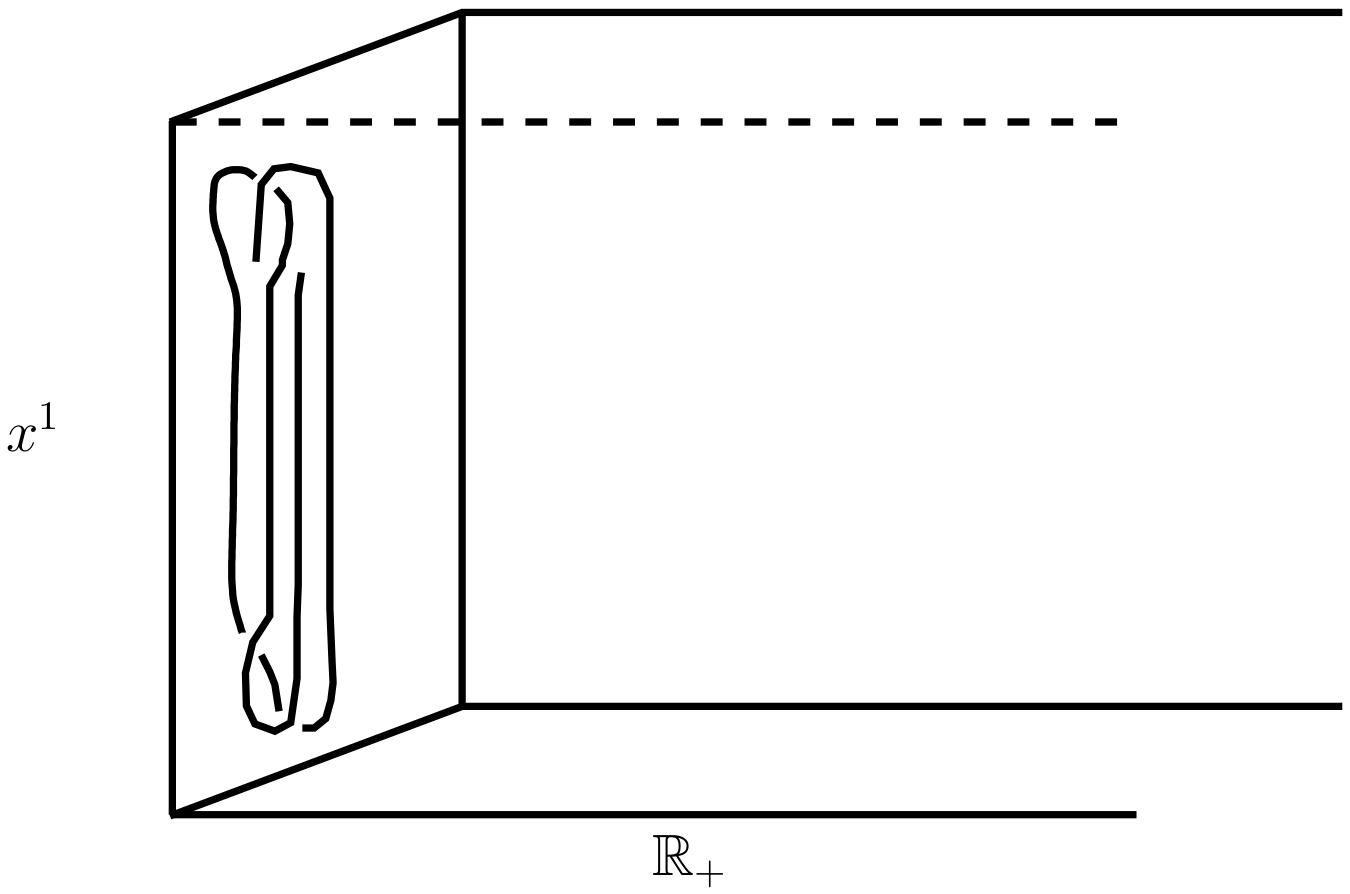
\includegraphics[width=3.5in]{figs/Fig02.png}
 \end{center}
\caption{\small   把一个纽结沿某一个方向——此处取为 $x^1$ 方向——拉伸，以约化为几乎处处近似与一个坐标无关的情形。经过充分拉伸之后，纽结处处近似与 $x^1$ 无关，唯一的例外是 $x^1$ 的有限个临界值附近，在那些地方一对股出现或消失。（在图中，这些只发生在顶部与底部。）（原稿第 9 页）}
 \label{stretching}
\end{figure}



第一个想法是拓扑场论中的标准想法。我们考虑 $W=\R\times C$ 中的纽结，其中 $C$（可以就是 $\R^2$）是一个二维流形，并用 $x^1$ 参数化 $\R$。我们把纽结沿 $x^1$ 方向拉伸，使得除了少数几个股数发生变化的例外 $x^1$ 值之外，边界条件几乎与 $x^1$ 无关（图~\ref{stretching}）。我们希望，在远离例外 $x^1$ 值的地方，解可以用与 $x^1$ 无关的解来逼近。一旦丢掉 $x^1$，方程就约化为三维中的方程。约化后的方程保持更多的超对称，人们可以期望理解它们的解。


\begin{figure}
 \begin{center}
     % >>> 原文图 3（原稿第 9 页）
  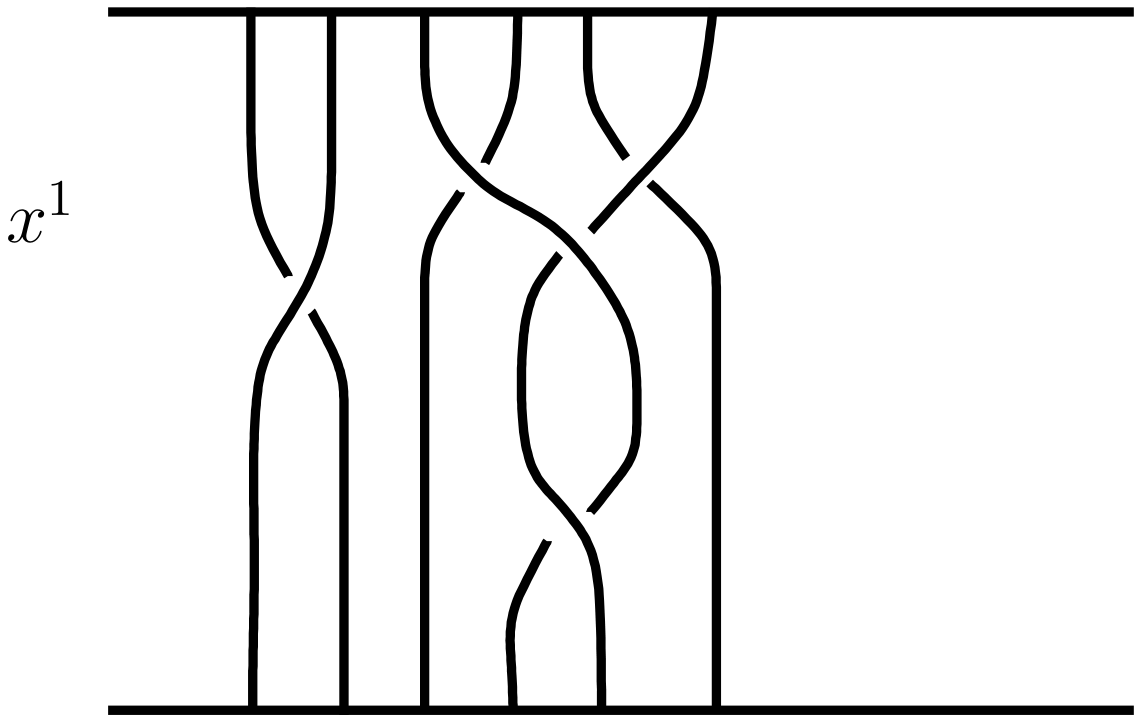
\includegraphics[width=3in]{figs/Fig03.png}
 \end{center}
\caption{\small  $I\times C$ 中的一个辫；把顶部与底部粘合起来，便可在 $S^1\times C$ 中得到一个闭合辫。经过充分拉伸后，一个辫可以用 $x^1$ 方向的绝热演化来描述，而不再有使这一描述失效的例外值。（原稿第 9 页）}
 \label{braid}
\end{figure}


在找到三维解之后，为恢复四维图像，我们必须考虑三维方程中参数的绝热变化。这是因为我们的纽结即使在拉伸之后也并非完全与 $x^1$ 无关。我们还必须考虑股数变化时发生的跳变。实际上，存在一个重要的特殊情形，其中只需考虑参数的绝热变化。这就是（图~\ref{braid}）把 $\R\times C$ 替换为  $S^1\times C$（或 $I\times C$，其中 $I$ 是闭区间，不过这会引入关于边界条件的问题）且把链环替换为辫的情形。在这种情况下，人们研究的将不是 Jones 多项式，而是与之相伴的辫群表示，后者同样极有意义。


\begin{figure}
 \begin{center}
     % >>> 原文图 4（原稿第 10 页）
  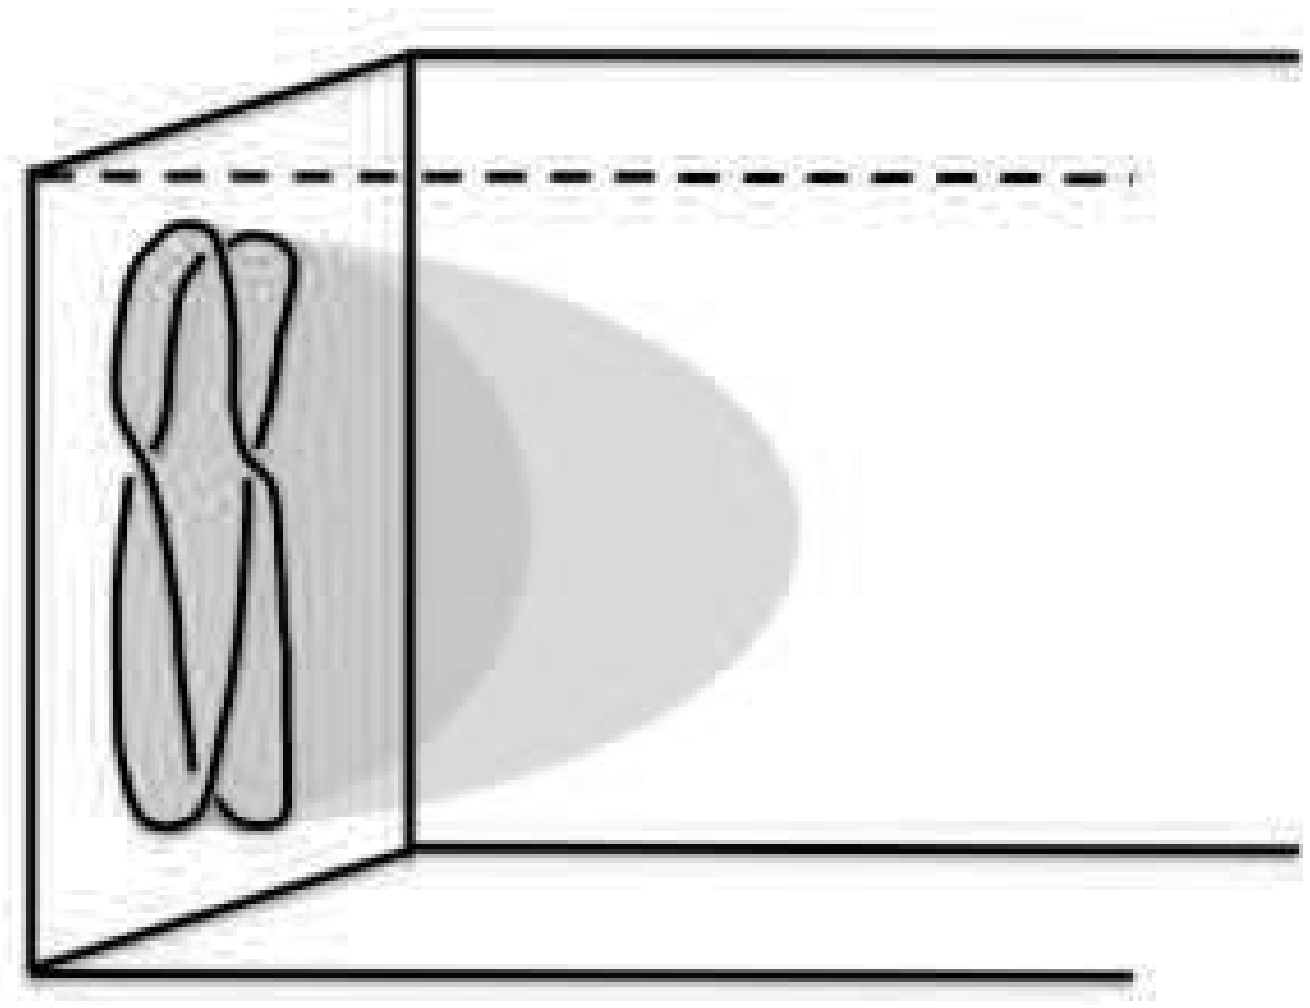
\includegraphics[width=3.5in]{figs/Fig04.png}
 \end{center}
\caption{\small  当纽结沿边界被拉伸时，超对称方程的解可能在垂直于边界的 $y$ 方向上变得离域化。图中示意性地表明了这一点；阴影区域表示解的空间延展范围——即该选定的解显著偏离无纽结时描述真空的解的区域——其厚度正比于纽结被拉伸的量。（原稿第 10 页）}
 \label{failure}
\end{figure}


关于这一方案，有一点重要之处需要提及：并不能保证它一定奏效。当把纽结沿 $x^1$ 方向拉伸时，解可能同时在 $y$ 方向上"铺展开"（图~\ref{failure}），以致即使在拉伸之后，解也可能不趋于与 $x^1$ 无关的极限。事实上，我们将发现这在某些条件下确实会发生。我们的主要任务之一，就是理解在什么条件下图~\ref{failure} 所暗示的那类行为不会发生。
% [Tutor Note: 物理图像] "铺展开"是本文的实质性困难：沿 x¹ 拉伸使边界条件的 x¹ 依赖变弱，但解在法向 y 上的尺度可能随拉伸而增大，从而不存在严格的 x¹ 无关极限。后文正是通过引入库仑分支参数破坏规范对称性、再把纽结放大到远大于 1/|a| 的尺度，来把 y 方向尺度压住；读者应把图~\ref{failure} 记作后文技术条件的直观来源。

在实施刚刚描述的方案时，我们从第~\ref{teqone}~节开始，取 $\t=\pm 1$，因为这对 Khovanov 同调是特殊取值（正如我们在上文第~\ref{lift}~节中所回顾的），也因为 $\t=\pm 1$ 时三维方程中的某些简化已在 \cite{fiveknots} 第 3.6 节中发现。

由于我们遇到了一些令人困惑的现象（最终我们将沿图~\ref{failure} 的思路理解它们），我们寻找一些额外的简化。在此过程中，我们主要利用两个想法。

第一个想法是修改边界条件以纳入规范对称性破缺。基本想法已在第~\ref{review}~节末尾解释过：我们不要求 $\vec\phi$ 在无穷远处为零，而要求 $\vec\phi\to g\vec \ca g^{-1}$，其中 $g\in G$，且 $\vec \ca=(\ca_1,\ca_2,\ca_3)$ 的三个分量取值于 $G$ 的李代数 $\frak g$ 的一个嘉当子代数中。（在更一般的情形 $W=\R\times C$ 中，我们会类似地修改边界条件，要求 $\phi$ 沿 $\R$ 方向的分量在无穷远处属于指定的共轭类。）以这种方式连续改变边界条件，应当不会改变导致 Jones 多项式的解的计数。另一方面，在此类计数问题中人们常发现，扰动到更一般的情形可以使问题变得更容易。此外，在目前的情形中，取 $\vec \ca$ 为一般的，会把我们所研究的非阿贝尔规范理论在低能下约化为阿贝尔理论。若我们把纽结放大，使 $K_i$ 的所有相关尺度都远大于 $1/|\vec \ca|$，那么我们有理由期望找到关于相关现象的某种有效阿贝尔描述。

第二个想法或许更加显然。由于在 $\t=1$ 时出现的、带上述 Nahm 极边界条件的方程相当特殊，我们扰动 $\t$ 的取值和/或 Nahm 极边界条件，使之变得更为一般。事实证明这非常富有成效，尤其是与规范对称性破缺结合时。

\subsection{结构与结果}\label{results}

在第~\ref{teqone}~节中，我们分析方程 (\ref{bpseqns}) 在 $\t=1$ 时的三维约化。我们得到以带某些附加结构的希格斯丛表述的有趣描述，但也清楚地看到，图~\ref{stretching} 所暗示的方案在 $\t=1$ 时会遇到一些困难。在第~\ref{analog}~节中，我们把方程扰动到 $\t\not=1$，并发现这为理解 Jones 多项式提供了有希望得多的框架。一般 $\t$ 的方程与数学物理中的多种课题有着出人意料且有用的联系，包括被称为 Gaudin 模型的可积自旋系统的 Bethe 方程，以及 Virasoro 代数某些特殊的"退化"共形块；本文余下部分就以这些联系为基础。在第~\ref{fourd}~节中，我们讨论由支配时间无关解的参数之绝热演化来构造辫群表示的一般框架。这一一般框架略显抽象，但在第~\ref{fthimconformal}~节中我们将证明，在我们的具体问题中，它可以借助某些 Virasoro 共形块的自由场表示而变得非常具体。在第~\ref{brrep}~节中，我们详细实施这一想法。这最终使我们能够理解如何通过计数四维 BPS 方程 (\ref{bpseqns}) 的解来恢复 Jones 多项式及与之相伴的辫群表示。第~\ref{supermon}~节致力于描述可用于理解第~\ref{teqone}~节与第~\ref{analog}~节某些微妙结果的、BPS 磁单极子的有效超势。在第~\ref{opbranes}~节中，我们把本文遇到的某些结构置于数学物理更宽广的语境中。三个附录补充推导的细节。
